% -----------------------------------------------------------------
% Document class: Article
\documentclass[ a4paper, twoside, 11pt]{article}
\usepackage{../../../macros-general}
\usepackage{../../../macros-article}
% Number of the handout, quiz, exam, etc.
\newcommand{\numero}{02}
\setcounter{numero}{\numero}

% -----------------------------------------------------------------
\begin{document}
\allowdisplaybreaks

\begin{center}
\Large Mec\'anica Vectorial (MECG-1001): Lecci\'on \numero \\[2ex]
\small \textbf{Semestre:} 2017-2018 T\'ermino II \qquad
\textbf{Instructor:} Luis I. Reyes Castro \qquad
\textbf{Paralelo:} 08
\end{center}
\fullskip

% =============================================
\begin{problem}
En el ensamble mostrado en la siguiente figura la barra $AB$ tiene una velocidad angular constante de 4 rad/s en el sentido de las manecillas del reloj. 

\begin{figure}[htb]
\centering
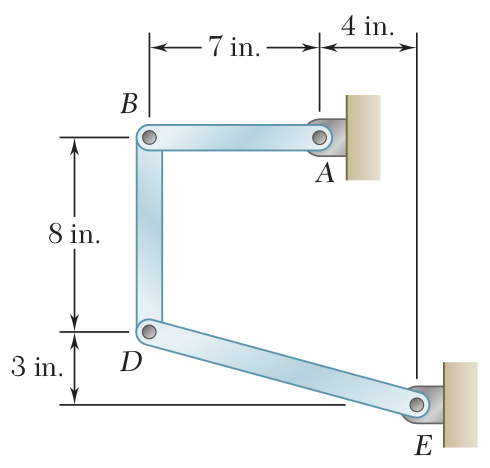
\includegraphics[width=0.38\textwidth]{problema-01.jpg}
\end{figure}

Complete las siguientes actividades: 
\begin{enumerate}[label=\textbf{\alph*)}]
\item \textbf{4 Puntos:} Encuentre las velocidades angulares de las barras $BD$ y $DE$. \\[1ex]
\emph{Soluci\'on:} Primero tomamos algunos datos: 
\begin{align*}
\vec{\hat{r}_{AB}} \; & = \; ( \, -1, \, 0 \, ) \\
\vec{r_{AB}} \; & = \; ( \, -7, \, 0 \, ) \; \text{in} \\
\vec{\hat{r}_{ED}} \; & = \; ( \, -0.9648, \, +0.2631 \, ) \\
\vec{r_{ED}} \; & = \; ( \, -11, \, +3 \, ) \; \text{in} \\
\vec{\hat{r}_{BD}} \; & = \; ( \, 0, \, -1 \, ) \\
\vec{r_{BD}} \; & = \; ( \, 0, \, -8 \, ) \; \text{in} \\
\vec{\omega_{AB}} \; & = \; -4 \; \uvec{k} \; \text{rad/s} \\
\vec{\alpha_{AB}} \; & = \; \vec{0} \; \text{rad/s\tsup{2}}
\end{align*}
Luego, reconocemos que las velocidades de $A$ y $B$ se relacionan con la velocidad angular de la barra $AB$ de la siguiente manera: 
\[
\vec{v_B}
\; = \; \vec{v_A} + \vec{\omega_{AB}} \cross \vec{r_{AB}}
\; = \; \colvec{0}{+28} \; \text{in/s}
\]
Similarmente, vemos que las velocidades de $D$ y $E$ se relacionan con la velocidad angular de la barra $DE$ de la siguiente manera: 
\[
\vec{v_D}
\; = \; \vec{v_E} + \vec{\omega_{DE}} \cross \vec{r_{ED}}
\; = \; \colvec{ -3 \, \omega_{DE}}{ -11 \, \omega_{DE}} \; \text{in/s}
\]
Finalmente, vemos que las velocidades de $B$ y $D$ se relacionan con la velocidad angular de la barra $BD$ de la siguiente manera: 
\begin{align*}
\vec{v_D} \;
& = \; \vec{v_B} + \vec{\omega_{BD}} \cross \vec{r_{BD}} \\
& = \; \colvec{0}{+28} + \colvec{ +8 \, \omega_{BD}}{0}
\; = \; \colvec{ +8 \, \omega_{BD}}{ +28} \; \text{in/s}
\end{align*}
Igualando las dos expresiones anteriores para la velocidad en $D$, tenemos: 
\begin{align*}
&
\colvec{ -3 \, \omega_{DE}}{ -11 \, \omega_{DE}}
\; = \; \colvec{ +8 \, \omega_{BD}}{ +28} \\
& \Longrightarrow \;
-11 \, \omega_{DE} \; = \; +28 \\
& \Longrightarrow \;
\vec{\omega_{DE}} \; = \; -2.546 \; \uvec{k} \; \text{rad/s} \\
& \Longrightarrow \;
\vec{\omega_{BD}} \; = \; +0.9546 \; \uvec{k} \; \text{rad/s}
\end{align*}

\item \textbf{4 Puntos:} Encuentre las aceleraciones angulares de las barras $BD$ y $DE$. \\[1ex]
\emph{Soluci\'on:} Primero, reconocemos que las aceleraciones de $A$ y $B$ se relacionan con la aceleraci\'on angular de la barra $AB$ de la siguiente manera: 
\begin{align*}
\vec{a_B} \;
& = \; \vec{a_A} + \vec{\alpha_{AB}} \cross \vec{r_{AB}} - \omega_{AB}^2 \, \vec{r_{AB}} \\
& = \; \vec{0} + \vec{0} -(-4)^2 \colvec{-7}{0} \; = \; \colvec{+112}{0} \; \text{in/s\tsup{2}}
\end{align*}
Similarmente, vemos que las aceleraciones de $D$ y $E$ se relacionan con la velocidad y aceleraci\'on angular de la barra $DE$ de la siguiente manera: 
\begin{align*}
\vec{a_D} \;
& = \; \vec{a_E} + \vec{\alpha_{DE}} \cross \vec{r_{ED}} - \omega_{DE}^2 \, \vec{r_{ED}} \\
& = \; \vec{0} + \colvec{ -3 \, \alpha_{DE}}{ -11 \, \alpha_{DE}} - (-2.546)^2 \, \colvec{-11}{+3} \\
& = \; 
\colvec{ +71.30 - 3 \, \alpha_{DE}}{ -19.47 - 11 \, \alpha_{DE}} \; \text{in/s\tsup{2}}
\end{align*}
Finalmente, vemos que las aceleraciones de $B$ y $D$ se relacionan con la velocidad y aceleraci\'on angular de la barra $BD$ de la siguiente manera: 
\begin{align*}
\vec{a_D} \;
& = \; \vec{a_B} + \vec{\alpha_{BD}} \cross \vec{r_{BD}} - \omega_{BD}^2 \, \vec{r_{BD}} \\
& = \; \colvec{+112}{0} + \colvec{ +8 \, \alpha_{BD}}{0} - (+0.9543)^2 \, \colvec{0}{-8} \\
& = \; 
\colvec{ +112 + 8 \, \alpha_{BD}}{+7.286} \; \text{ft/s\tsup{2}}
\end{align*}
Igualando las dos expresiones anteriores para la aceleraci\'on en $D$, tenemos: 
\begin{align*}
&
\colvec{ +71.30 - 3 \, \alpha_{DE}}{ -19.47 - 11 \, \alpha_{DE}} \; = \; \colvec{ +112 + 8 \, \alpha_{BD}}{+7.286} \\
& \Longrightarrow \;
-19.47 - 11 \, \alpha_{DE} \; = \; +7.286 \\
& \Longrightarrow \;
\vec{\alpha_{DE}} \; = \; -2.4324 \; \uvec{k} \; \text{rad/s\tsup{2}} \\
& \Longrightarrow \;
\vec{\alpha_{BD}} \; = \; -4.1754 \; \uvec{k} \; \text{rad/s\tsup{2}}
\end{align*}
\QED

\end{enumerate}

\end{problem}
\fullskip

% =============================================
\begin{problem}
\textbf{[6 Puntos]} Dos discos uniformes y dos cilindros est\'an ensamblados de la manera como se muestra en la siguiente figura. El disco $A$ pesa 20 lb y el disco $B$ pesa 12 lb. Si el sistema se suelta desde el reposo, encuentre las aceleraciones angulares de los discos y las aceleraciones translacionales de los cilindros. 

\begin{figure}[H]
\centering
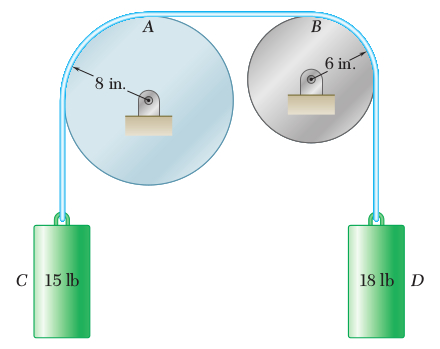
\includegraphics[width=0.50\textwidth]{problema-02.jpg}
\end{figure}

\emph{Soluci\'on:} Primero tomamos algunos datos: 
\begin{align*}
m_A \; & = \; 0.6216 \; \text{slug} \\
m_B \; & = \; 0.3730 \; \text{slug} \\
m_C \; & = \; 0.4662 \; \text{slug} \\
m_D \; & = \; 0.5595 \; \text{slug} \\
I_A \; & = \; (1/2) \, m_A \, r_A^2 \; = \; 0.1381 \; \text{slug-ft\tsup{2}} \\
I_B \; & = \; (1/2) \, m_B \, r_B^2 \; = \; 0.0466 \; \text{slug-ft\tsup{2}}
\end{align*}
Ahora, si definimos a las tensiones de la cuerda en los segmentos $AC$, $AB$ y $BD$ como $T_{AC}$, $T_{AB}$ y $T_{BD}$, respectivamente, entonces podemos ver que las sumatorias de torques en las poleas y las sumatorias de fuerzas en los cilindros resultan en: 
\begin{align*}
& I_A \, \alpha_A \; = \; +r_A \, ( T_{AC} - T_{AB} ) \\
& I_B \, \alpha_B \; = \; +r_B \, ( T_{AB} - T_{BD} ) \\
& m_C \, (\vec{a_C})_y \; = \; +T_{AC} - W_C \\
& m_D \, (\vec{a_D})_y \; = \; +T_{BD} - W_D
\end{align*}
Para simplificar estas ecuaciones reconocemos las siguientes restricciones cinem\'aticas: 
\begin{align*}
r_A \, \alpha_A \; & = \; r_B \, \alpha_B
\quad \Longrightarrow \quad
\alpha_B \; = \; (4/3) \, \alpha_A \; \text{rad/s\tsup{2}} \\
(\vec{a_C})_y \; & = \; -r_A \, \alpha_A
\quad \Longrightarrow \quad
(\vec{a_C})_y \; = \; -(2/3) \, \alpha_A \; \text{ft/s\tsup{2}} \\
(\vec{a_D})_y \; & = \; +r_B \, \alpha_B
\quad \Longrightarrow \quad
(\vec{a_D})_y \; = \; +(2/3) \, \alpha_A \; \text{ft/s\tsup{2}}
\end{align*}
Reemplazando $\alpha_B$, $(\vec{a_C})_y$ y $(\vec{a_D})_y$ en las sumatorias de torques y fuerzas, obtenemos el siguiente sistema de cuatro ecuaciones en las cuatro inc\'ognitas $\alpha_A$, $T_{AC}$, $T_{AB}$ y $T_{BD}$, tal como se muestra a continuaci\'on. 
\begin{align*}
& I_A \, \alpha_A \; = \; +(2/3) \, ( T_{AC} - T_{AB} ) \\
& (4/3) \, I_B \, \alpha_A \; = \; +(1/2) \, ( T_{AB} - T_{BD} ) \\
& -(2/3) \, m_C \, \alpha_A \; = \; +T_{AC} - W_C \\
& +(2/3) \, m_D \, \alpha_A \; = \; +T_{BD} - W_D
\end{align*}
Resolviendo este sistema para la aceleraci\'on angular de la polea obtenemos: 
\[
\vec{\alpha_A} \; = \; -1.724 \; \uvec{k} \; \text{rad/s\tsup{2}}
\]
Consecuentemente: 
\begin{align*}
\vec{\alpha_B} \; & = \; -2.299 \; \uvec{k} \; \text{rad/s\tsup{2}} \\
\vec{a_C} \; & = \; +1.149 \; \uvec{j} \; \text{ft/s\tsup{2}} \\
\vec{a_D} \; & = \; -1.149 \; \uvec{j} \; \text{ft/s\tsup{2}}
\end{align*}
\QED

\end{problem}
\fullskip

% =============================================
\begin{problem}
\textbf{[4 Puntos]} La plataforma de 9 kg est\'a soportada, como se muestra en la siguiente figura, por dos discos uniformes que ruedan sin deslizarse en todas las superficies de contacto. La masa de cada disco es de 6 kg y el radio de 80 mm. Si se sabe que el sistema est\'a inicialmente en reposo, determine la velocidad de la plataforma despu\'es de que \'esta se haya desplazado 250 mm. 

\begin{figure}[htb]
\centering
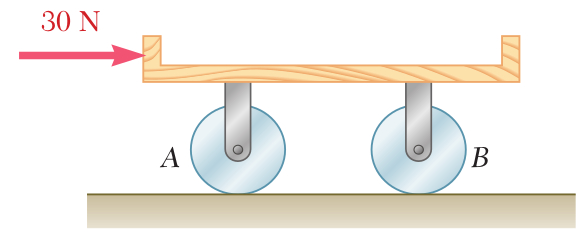
\includegraphics[width=0.5\textwidth]{problema-03.jpg}
\end{figure}

\emph{Soluci\'on:} Puesto que el sistema parte del reposo y que no hay cambios en su energ\'ia potencial, vemos que el trabajo externo causado por la fuerza $F = 30$ N al desplazar el centro de masa del sistema $\delta = 0.250$ m debe ser igual a la energ\'ia cin\'etica total del sistema despu\'es del desplazamiento. El trabajo externo es: 
\[
\Delta E_{12} \; = \; F \, \delta \; = \; 7.5 \; \text{J}
\]
La energ\'ia cin\'etica total es la suma de la energ\'ia cin\'etica translacional de la plataforma con las energ\'ia cin\'eticas translacionales y rotacionales de los discos. Definiendo a $v_P$ como la velocidad de la plataforma, a $v_D$ como la velocidad del centro de masa de cada disco, y a $\omega_D$ como la velocidad angular de cada disco, tenemos: 
\[
E_2 \; = \; K_2 \; = \; 
(1/2) \, m_P \, v_P^2 + (2) \, [ \, (1/2) \, m_D \, v_D^2 + (1/2) \, I_D \, \omega_D^2 \, ]
\]
Ahora aplicamos consideraciones cinem\'aticas. Claramente $v_P = v_D$. Adem\'as, por la condici\'on de rodadura tenemos $v_D = r_D \, \omega_D$, por lo que $\omega_D = v_P / r_D$. Recordando tambi\'en que la inercia de cada disco es $I_D \; = \; (1/2) \, m_D \, r_D^2$, la energ\'ia en el segundo estado es: 
\begin{align*}
E_2 \;
& = \; (1/2) \, m_P \, v_P^2 + (2) \, [ \, (1/2) \, m_D \, v_P^2 + (1/2) \, I_D \, ( v_P / r_D )^2 \, ] \\
& = \; [ \, (1/2) \, m_P + m_D + ( I_D / r_D^2 ) \, ] \, v_P^2 \\
& = \; [ \, (1/2) \, m_P + (3/2) \, m_D \, ] \, v_P^2 \\
& = \; 40.5 \, v_P^2
\end{align*}
Finalmente, aplicando el Principio Trabajo-Energ\'ia, tenemos que $E_2 = \Delta E_{12}$. Igualando estas dos expresiones y resolviendo para $v_P$ concluimos que: 
\[
\vec{v_P} \; = \; +0.4303 \; \uvec{i} \; \text{m/s}
\; \equiv \; +430.3 \; \uvec{i} \; \text{mm/s}
\]
\QED

\end{problem}
\fullskip

% =============================================
\begin{problem}
Dos barras ligeras id\'enticas $AB$ y $BC$ se sueldan entre si para formar un mecanismo en forma de $L$, el cual se presiona contra un resorte en $D$ y se suelta desde la posici\'on indicada, tal como se muestra en la siguiente figura. Se sabe que el \'angulo m\'aximo de rotaci\'on del mecanismo en su movimiento subsecuente es de 90\deg en sentido contrario al de las manecillas del reloj. 

\begin{figure}[H]
\centering
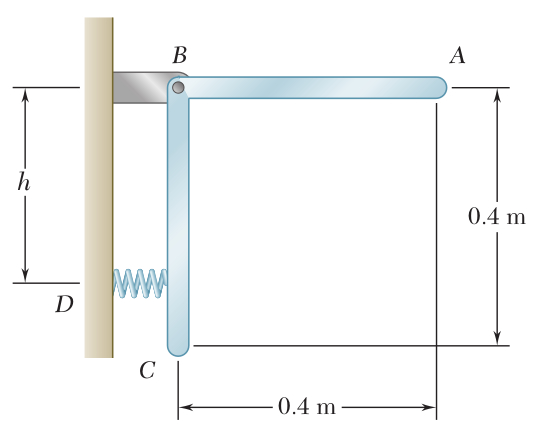
\includegraphics[width=0.4\textwidth]{problema-04.jpg}
\end{figure}

Complete las siguientes actividades: 
\begin{enumerate}[label=\textbf{\alph*)}]
\item \textbf{1 Punto:} Calcule la inercia del ensamble alrededor de $B$. \\[1ex] \emph{Soluci\'on:} Suponiendo que la masa de cada barra es $m$, tenemos: 
\[
I_B \; = \; 
(2) \, (1/12) \, m \, \ell^2 + (2) \, m \, (\ell/2)^2
\; = \; (2/3) \, m \, \ell^2
\; = \; 0.1067 \, (m) \; \text{kg-m\tsup{2}}
\]
En cambio, si suponemos que la masa del ensamble es $M$, tenemos: 
\[
I_B \; = \; (2/3) \, (M/2) \, \ell^2
\; = \; (1/3) \, M \, \ell^2
\; = \; 0.0533 \, (M) \; \text{kg-m\tsup{2}}
\]

\item \textbf{5 Puntos:} Determine la magnitud de la velocidad angular del mecanismo cuando pasa por la posici\'on en la que la barra $AB$ forma un \'angulo de 30\deg con la horizontal. \\[1ex]
\emph{Soluci\'on:} Definimos el primer estado como aquel donde la barra $AB$ est\'a en posici\'on vertical, es decir, donde alcanza su \'angulo, y el segundo estado donde la misma barra forma un \'angulo de $\theta = 30\deg$ con la horizontal. Con esto en mente, primero computamos el centro de masa del ensamble con respecto al punto $B$. Por simetr\'ia, es evidente que en la posici\'on mostrada en la figura el centro de masa del ensamble se localiza en el punto $\vec{G_0} = (+\delta,-\delta)$, donde: 
\[
\delta \; = \; 
\frac{(m)(\pm 0) + (m)(+\ell/2)}{2m} \; = \; +0.1 \; \text{m}
\]
De este c\'alculo tambi\'en podemos reconocer que punto $B$ siempre se encuentra a una distancia de $r = \delta \sqrt{2}$ m del centro de masa del ensamble. Adicionalmente, podemos observar que en el primer estado la locaci\'on del centro de masa del ensamble es $\vec{G_1} = (+0.1,+0.1)$, mientras que en el segundo estado es: 
\[
(\vec{G_2})_y \; = \;
\frac{ (m)[ (+\ell/2) \sin(30\deg) ] + (m)[ (-\ell/2) \cos(30\deg)] }{2m}
\; = \; -0.0366 \; \text{m}
\]
Vemos as\'i que la altura del centro de masa del ensamble en el primer estado relativo al segundo estado es: 
\[
h \; = \; (\vec{G_1})_y - (\vec{G_2})_y
\; = \; (+0.1) - (-0.0366) \; = \; +0.1366 \; \text{m}
\]
Consecuentemente, la energ\'ia del sistema en el primer estado es: 
\[
E_1 \; = \; U_1 \; = \; (2m) \, g \, h \; = \; 2.68 \, (m) \; \text{J}
\]
Mientras que la energ\'ia del sistema en el segundo estado es: 
\begin{align*}
E_2 \; = \; K_2 \;
& = \;
(1/2) \, (2m) \, (v_G)^2 + (1/2) \, I_B \, \omega^2 \\
& = \;
m \, (v_G)^2 + (1/3) \, m \, \ell^2 \, \omega^2
\end{align*}
Ahora, puesto que el ensamble est\'a rotando alrededor del punto $B$ es evidente que $v_G = r \, \omega = \delta \, \sqrt{2} \, \omega$. Esto implica que: 
\begin{align*}
E_2 \; = \; K_2 \;
& = \; [ \, m \, (\delta \sqrt{2})^2 + (1/3) \, m \, \ell^2 \, ] \, \omega^2 \\
& = \; [ \, 2 \, m \, \delta^2 + (1/3) \, m \, \ell^2 \, ] \, \omega^2
\; = \; 0.0733 \, (m) \, (\omega^2) \; \text{J}
\end{align*}
Finalmente, aplicamos el Principio Trabajo-Energ\'ia. Puesto que nunca act\'uan fuerzas externas no-conservativas, la energ\'ia no puede cambiar entre estados, \ie $E_1 = E_2$. Igualando las dos expresiones vemos que se cancelan las masas de las barras y que la velocidad angular del ensamble es: 
\[
\omega \; = \; \pm 6.047 \; \uvec{k} \; \text{rad/s}
\]
La direcci\'on exacta depende de si usted consider\'o en ensamble mientras sub\'ia o mientras o bajaba, y por lo tanto es irrelevante. 
\QED

\end{enumerate}

\end{problem}
\fullskip

\end{document}